% !TEX root = ../main.tex

\chapter{平衡拉丁方排序设计}

为进一步控制呈现顺序带来的偏差,我们设计并实施了用户研究的另一版本,采用 HCI 用户研究工具包 \cite{LatinSquareToolkit} 生成的平衡拉丁方(Balanced Latin Square)排序。本实验版本共招募 8 位参与者(4 名男性,4 名女性),全部使用 VR 头显设备,以构建性别平衡的样本组。如图~\ref{fig:userstudy_latin_square} 所示,展示了该版本用户在“真实感”、“同步性”和“多样性”三个维度上的评分结果。

\begin{figure}[h]
\centering
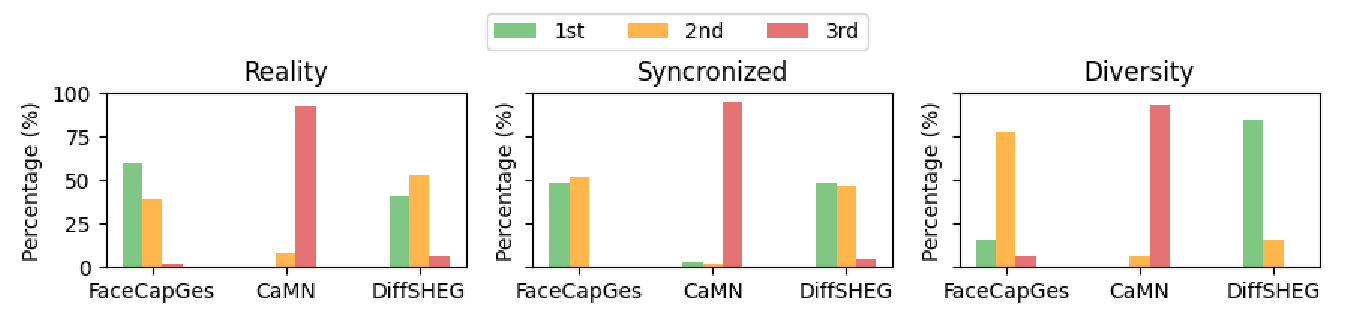
\includegraphics[width=\linewidth]{figures/UserStudy_LatinSquare.png}
\caption{平衡拉丁方实验版本中的用户主观评分结果,共 8 位参与者,评价维度包括“真实感”、“同步性”和“多样性”。}
\label{fig:userstudy_latin_square}
\end{figure}

本研究中所用播放界面如图~\ref{fig:userstudy_app} 所示。该界面在 VR 与桌面端中保持一致,使参与者能够以随机顺序观看三种模型(FaceCapGes(本方法)、DiffSHEG \cite{diffsheg}、CaMN \cite{beatcamn})生成的手势动画。用户可多次重播当前片段,但不能返回浏览先前内容。在每段视频播放结束后,参与者通过拖动界面下方的评分面板,对三个模型进行排序打分。该界面同样适用于平衡拉丁方实验版本,确保所有参与者使用统一的评估流程。

\begin{figure}[h]
\centering
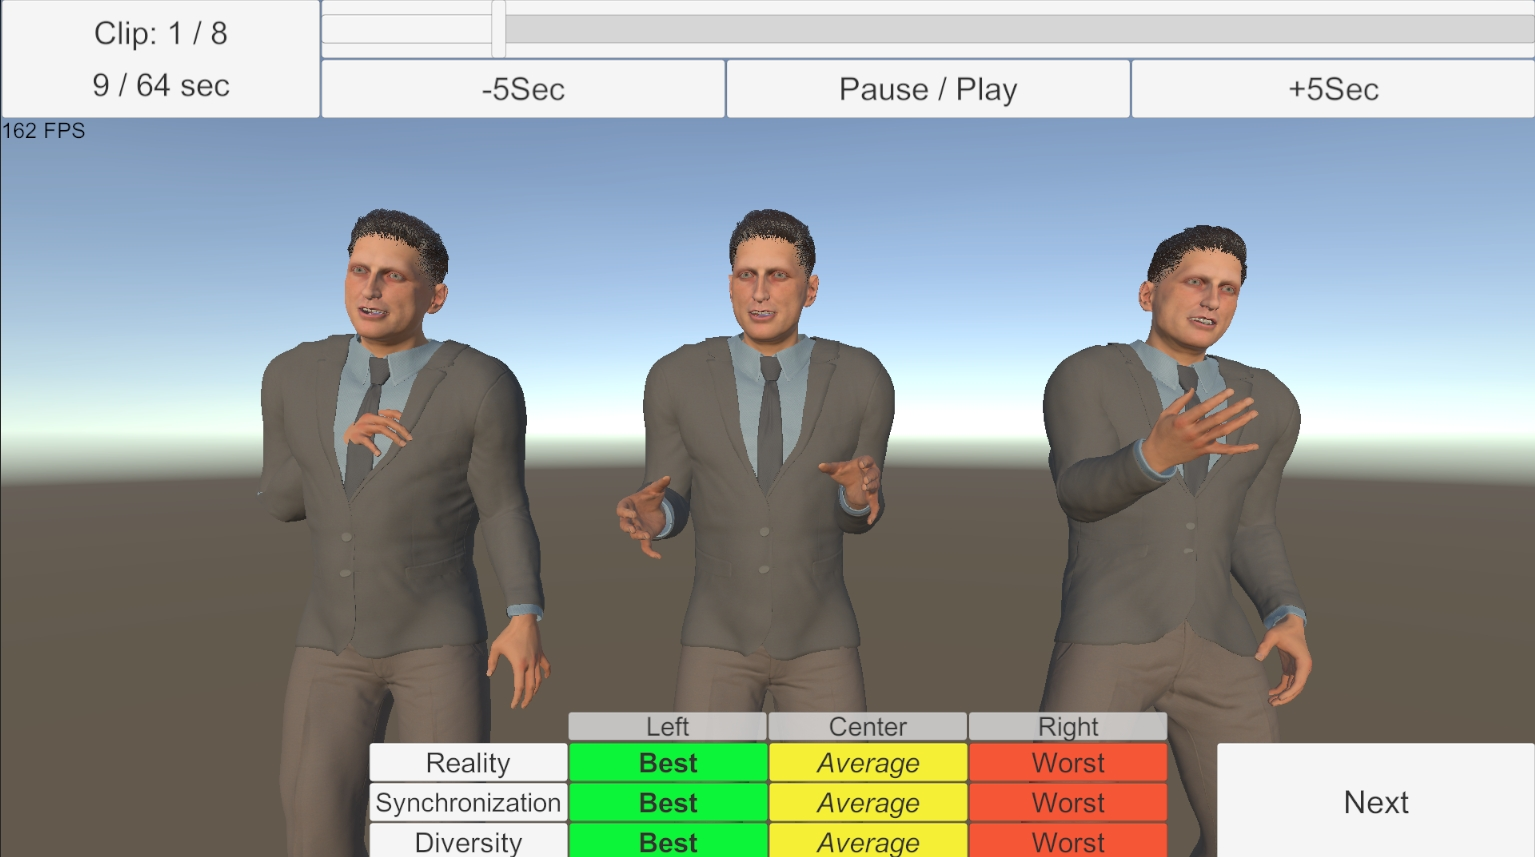
\includegraphics[width=\linewidth]{figures/UserStudyImage.png}
\caption{用户研究中使用的手势播放界面示意图。}
\label{fig:userstudy_app}
\end{figure}
